\chapter{Implementation}
\label{chap:implementation}

%%%%%%%%%%%%%%%%%%%%%%%%%%%%%%%%%%%%%%%%%%%%%%%%%%%%%%%%%%%%%%%%%%%%%%%%%%%%%%%%%%%%%%%%%%%%%%%%%%%%

This chapter will document the implementation process of the robot's systems. Rather than elaborating on trivial code specifics, the discussion will cover the various interactions between nodes and their topics.

%%%%%%%%%%%%%%%%%%%%%%%%%%%%%%%%%%%%%%%%%%%%%%%%%%%%%%%%%%%%%%%%%%%%%%%%%%%%%%%%%%%%%%%%%%%%%%%%%%%%

\section{Hardware Operation}

\subsection{RGB-D Camera Driver}

A wrapper for the \emph{OpenNI2} library is provided by the \texttt{openni2\_camera} \cite{ros_wiki_openni2_camera} and \texttt{openni2\_launch} \cite{ros_wiki_openni2_launch} packages. The former provides a single nodelet which acquires and publishes the image data, whereas the latter provides a means for starting that nodelet.

This driver publishes image data from the camera on a number of different topics, with varying data types. Only two of these are particularly useful to us, however. The topic \texttt{/camera/rgb/image} provides the general optical feed from the camera, and the topic \texttt{/camera/depth/image} provides the depth feed from the camera, both of message type \texttt{Image}. An example of the output from these topics is shown in \autoref{fig:rgbd_images1}. While the depth feed can be interpreted as an 8-bit monochrome image for displaying on-screen, the image is actually given in a 16-bit format, where each pixel value represents the distance from the sensor in millimeters. Additionally, the depth data is available in a point cloud format, published on \texttt{/camera/depth/points} as \texttt{PointCloud2} messages. This can be visualised in RViz, an example of which is shown in \autoref{fig:rgbd_images2}.

\begin{figure}[!h]
    \centering
    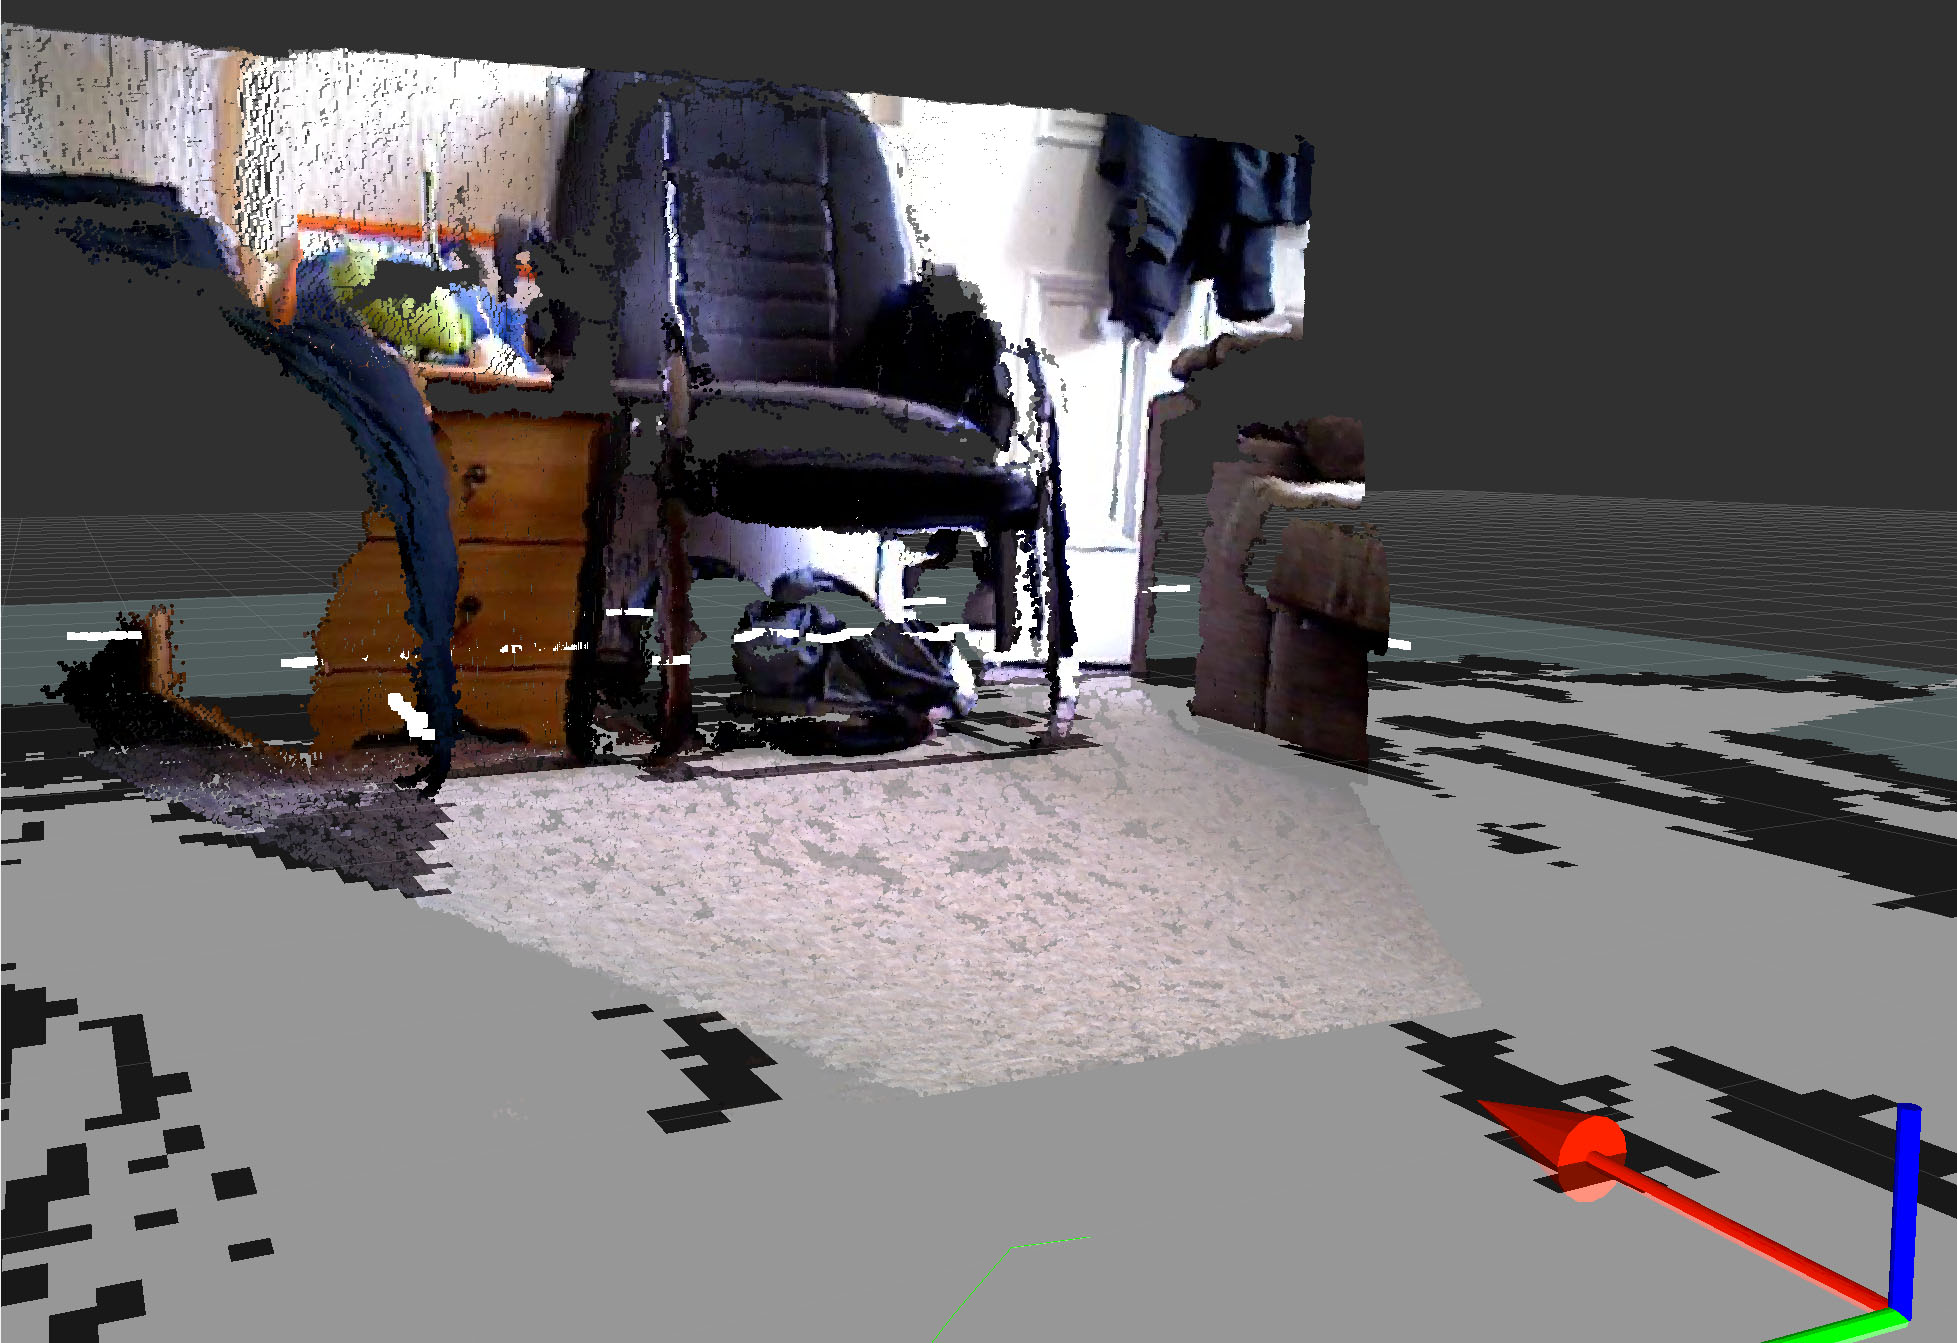
\includegraphics[width=12cm]{rgbd_pc2.jpg}
    \caption{Example point cloud output from the RGB-D camera mounted on top of the robot, as given by the \texttt{openni2\_camera} package, visualized using RViz. In this case, the points are projected into 3D space relative to the robot's position, and then coloured using the corresponding pixels on the RGB image.}
    \label{fig:rgbd_images2}
\end{figure}

The \texttt{openni2\_launch} package also publishes static TF transforms for the individual sensors on the camera, such that the slight differences in perspective can be corrected.

Camera calibration is also performed.

Understanding these package was rather troublesome, as both the wiki and GitHub pages documenting them were (and still are) completely blank. Instead, the documentation for a similar set of these packages for the first version of \emph{OpenNI}, named \texttt{openni\_launch}, was used \cite{ros_wiki_openni_launch}. Regardless, there was little difficulty in integrates this package due the little configuration it requires.

\subsection{Servo Driver}

While there were already drivers available for the RGB-D sensor, this was not the case for the servo controller. A custom \texttt{servo\_controller} node was developed which accepts command messages through a topic. This node then relays commands to the controller by converting them into the format specified in the protocol. Furthermore, the node is implemented in such a way that it can be used to move any number of servos connected to the controller, not just the eighteen as required by the hexapod.

The node listens for movement commands on a topic named \texttt{direct} relative to its namespace. By using a topic over a service, we ensure that any node sending commands to the controller need not wait for the command to actually be issued. This simplifies any timing necessities for a commanding node, such as those performing locomotion duties. A custom \texttt{ServoCommand} message had to be created to support this topic as none of the standard messages distributed with ROS were appropriate. In particular, it was necessary that a command include which servo to rotate, the target position, and how long it should take to move to that angle. The specification for this message is shown in \autoref{fig:servocommand_msg}. Having received one of these messages, the node will relay it to the controller after performing the steps necessary to transform it into the required protocol format.

\begin{figure}[!h]
	\centering
	\begin{tabular}{ r r p{12cm} }
		\textbf{Name} & 
		\textbf{Type} & 
		\textbf{Description} \\
		\hline

		\texttt{index} & 
		\texttt{uint8} &
		An index indicating which servo to rotate, where $0 \leq i \leq 31$. \\
		
		\texttt{angle} & 
		\texttt{int16} & 
		The target position that the servo should rotate to in degrees, generally where $0 \leq \theta \leq 180$. This can also accept negative values such that it can be used for supplying servo offsets. \\
		
		\texttt{duration} &
		\texttt{float32} &
		The duration for how long the rotation should take in seconds, essentially setting a speed for the rotation. \\
	\end{tabular}
	\caption{The specification for the \texttt{ServoCommand} message as used by the \texttt{servo\_controller} node. A \texttt{header} field is also included but omitted for brevity.}
	\label{fig:servocommand_msg}
\end{figure}

To specify the time taken to rotate the servo, a \texttt{duration} primitive could have been used rather than a \texttt{float32} \cite{ros_wiki_msg}. These primitives are by backed by classes in the client libraries such that they can be manipulated more easily \cite{ros_api_duration_msg}. For example, a \texttt{duration} can be added to a \texttt{time}---another primitive---resulting in a new \texttt{time}. While this may be useful, the duration can only be specified using integers in either \emph{seconds} or \emph{nanoseconds} \cite{ros_api_duration_msg}. This granularity can be quite tedious as the rotation durations are usually specified in the range of hundreds of milliseconds. To give an example, to rotate with a duration of a 0.1 seconds, the duration would need to be specified as either 1 second---thus being wildly inaccurate---or 100,000,000 nanoseconds---a rather excessively large number. It was for this reason that \texttt{float32} was chosen as it allows time to specified in seconds directly with fractions if necessary.

As standard with UNIX systems, the device presents itself as a file located in the \texttt{/dev} directory once connected which can be read from and written to \cite{unix_devices}. In this case, the device shows itself to be an external serial port with path \texttt{/dev/ttyAMC0} though this may vary depending on system configuration. While it is possible to open this file and begin writing directly using standard Python file semantics, a number of settings must be applied beforehand to ensure correct operation. A library named \emph{pySerial} was used to simplify this process by encapsulating access to the serial port while still a means of reading and writing using the familiar file semantics \cite{pyserial}. Additionally, this library provides the same interface to the serial port across many platforms allowing the controller node to be used in a variety of situations \cite{pyserial}.

A number of calculations must be performed to convert the supplied \texttt{ServoCommand} message into the right format for the protocol. Firstly, the protocol mandates that servo indices begin from 1, rather than 0. For this, we simply increment the supplied \texttt{index} by 1. Secondly, the target position sent to the controller must be a PWM duration where 1.5\textmu{}s corresponds to 0\textdegree{} and 2.5\textmu{}s corresponds to 180\textdegree{}. As we know the supplied \texttt{angle} will fall between 0 and 180, we can apply formula to get the correct value, specifically $1500 + (\theta / 180 * 1000)$. Finally, the protocol expects the duration to be an integer representing number of milliseconds. This conversion is achieved by simply multiplying the value by 1000, converting the supplied \texttt{duration} field from seconds to milliseconds.

Due to some quirk in the servo controller's programming, a time delay had to be added between sending commands. Without this, commands would get lost or abort midway through a rotation. A delay of 3 milliseconds was adequate to correct this without causing timing issues elsewhere in the system, minimized purely through trial and error. Seemingly, the controller requires some processing time after a command before it can begin processing another. Unfortunately, it is impossible to diagnose this issue any further as no source code is available, nor does the protocol documentation mention this limitation in any form \cite{torobot_manual}.

%%%%%%%%%%%%%%%%%%%%%%%%%%%%%%%%%%%%%%%%%%%%%%%%%%%%%%%%%%%%%%%%%%%%%%%%%%%%%%%%%%%%%%%%%%%%%%%%%%%%

\section{Locomotion}

\subsection{Limb Controller}

To simplify joint control, a further layer of abstraction atop the \texttt{servo\_controller} node was added. This layer of abstraction divides the servos into logical groupings based on the particular limb and limb section (i.e., foot, shin, body). Without this abstraction, any commanding node would need to calculate the correct servo index based on what limb and which part of the limb it wished to rotate. A custom \texttt{limb\_controller} node was implemented to provide these groupings, taking away the burden of any calculation. Furthermore, angle offsets and inversion flags can be supplied per-servo through this node, providing a means of calibration. This node essentially acts as a proxy for the \texttt{servo\_controller} node, modifying the messages as necessary.

The \texttt{limb\_controller} node listens for \texttt{ServoCommand} messages on three topics relative to itself. These topics are \texttt{/joint/body}, \texttt{/joint/shin}, and \texttt{/joint/foot}, each controlling the body, shin, and foot sections respectively. When a message is received on these topics, a new \texttt{ServoCommand} message is created with correct servo index and any angle adjustments. This is then sent to the \texttt{servo\_controller} node to control the requested limb section proper.

\begin{figure}[!h]
    \centering
    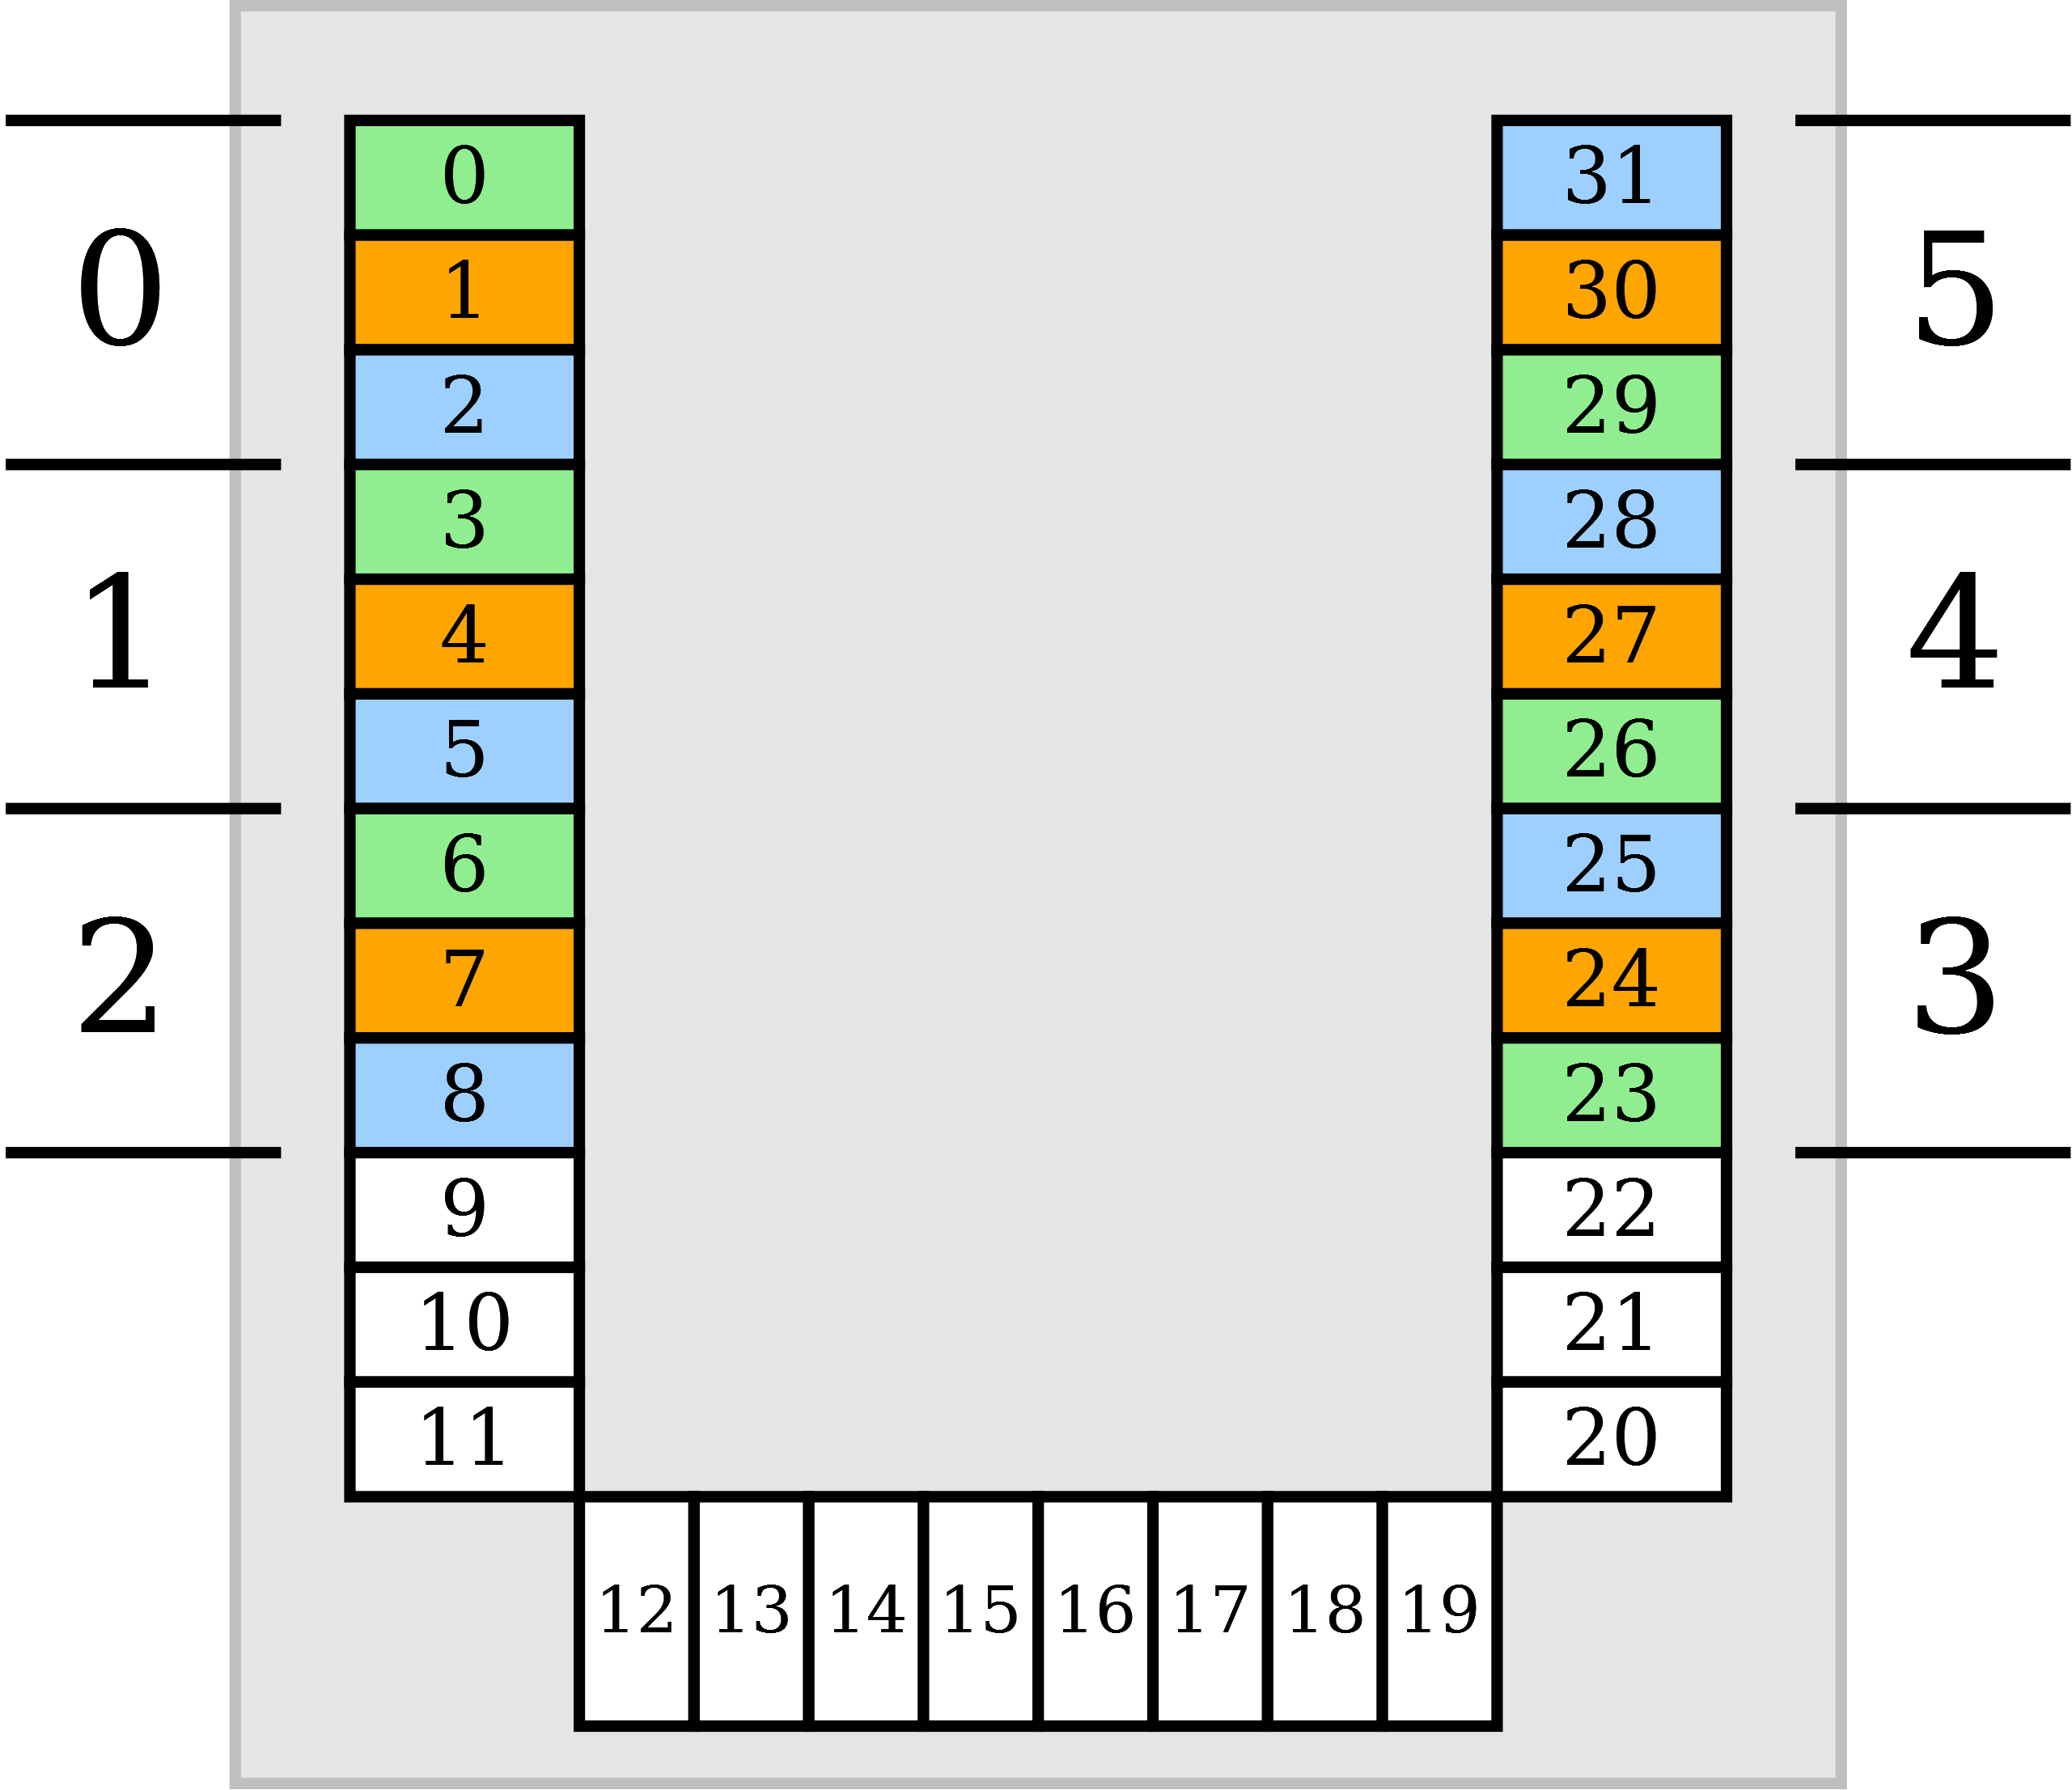
\includegraphics[width=8cm]{limb_controller.png}
    \caption{A simplified diagram showing where each servo on the robot is connected to the servo controller along with their corresponding limb number. Green boxes represent body joint servos, orange boxes represent shin joint servos, and blue boxes represent foot joint servos. White boxes represent unoccupied connections. Connecting the servos in this way allows for better cable management as well as giving the largest amount of cable slack to each limb.}
    \label{fig:servo_pins}
\end{figure}

Some logic and arithmetic must be performed to calculate the correct servo index for a given limb index and limb section. A diagram showing how the servos are connected to the servo controller is shown in \autoref{fig:servo_pins}. From this, it can be seen that servos are grouped per limb and then ordered by particular limb section. For a given limb index $i$, the servo index of the first joint in the grouping---the body joint---can be calculated by the formula $s = i * 3$. Then, a further displacement can be added to find the servo index of the other joints. To find the servo index of the shin joint we calculate $s = s + 1$, and to find the servo index of foot joint we calculate $s = s + 2$. While these formulae gives the correct indices for the first three limbs, we must also take into account the fact that the remaining three limbs begin at a servo index of 23 rather than 0. A trivial piece of logic to deal with this was added which simply increments the final servo index by 23 should the supplied limb be on that side. A code snippet is shown in \autoref{fig:actual_index} showing the specifics of how this is calculated.

\begin{figure}[!h]
    \centering
	\begin{lstlisting}[language=Python]
	def __actual_index(index, offset):
		actual_index = ((index % 3) * 3) + offset
		if index >= 3:
			actual_index += (31 - 8)

		return actual_index
	\end{lstlisting}
	\caption{A code snippet from the \texttt{limb\_controller} node showing how servo indices are calculated.}
	\label{fig:actual_index}
\end{figure}

For calibration, the \texttt{limb\_controller} node listens on a further three topics relative to itself, with similar paths as the movement topics. These topics are \texttt{/joint/offset/body}, \texttt{/joint/offset/shin}, and \texttt{/joint/offset/foot}. These topics also use the \texttt{ServoCommand} message, simply ignoring the \texttt{duration}. This allows offsets to be changed at run-time. When a message is received on these topics, the offset of that particular servo is registered but does not take effect until next time the servo moves. This is because the current servo positions are not tracked by the \texttt{limb\_controller} node so no updates can be made.

In addition to these offset topics, functionality for loading a data file containing the servo offsets was also implemented. An \texttt{offsets\_path} parameter can be supplied to specify where this file is located. This file is loaded upon launching the \texttt{limb\_controller} node, meaning that any movements will immediately take the offsets into account. The \texttt{pickle} module---part of Python's standard library---was used to support the loading of this data file \cite{pickle}. The specifics of this are explained in the next subsection.

\subsection{Limb Calibration Tool}

An interactive \texttt{limb\_calibrator} node was created to assist in the calibration of the limb sections. This takes form of a terminal application which allows the user to adjust joint offsets using the arrow keys on the keyboard. While running, the currently selected limb and limb section is displayed on-screen, along with its current offset. The user can select which joint section they wish to manipulate using a number of hotkeys. The resulting offsets can then be saved to a data file, which can be loaded automatically by the \texttt{limb\_controller} node on system launch. An example of the output provided by the node is shown in \autoref{fig:joint_calibrator_out}.

\begin{figure}[!h]
    \centering
	\begin{lstlisting}
	Offset: -5
	Joint: B
	Limb: 0
	\end{lstlisting}
	\caption{An example of the output given by the \texttt{limb\_calibrator} node. This is displayed in the terminal in which the node is ran, and updates as the user provides keyboard input.}
	\label{fig:joint_calibrator_out}
\end{figure}

All input is provided by keyboard key presses. The user can alter which limb is currently selected  by using the \emph{left} and \emph{right} arrow keys. The user can increment and decrement the offset of the currently selected joint by pressing the \emph{up} and \emph{down} arrow keys respectively. Joint section is made using the \emph{b}, \emph{s}, and \emph{f} keys, which select the body, shin and foot joints respectively. Pressing the \emph{l} key will load a saved offset file, and pressing the \emph{x} key will save the current offsets to a data file. The program can be exited by pressing the \emph{q} key.

Each time an adjustment is made, the node sends \texttt{ServoCommand} messages on the offset topic matching the currently selected joint, as required by the \texttt{limb\_controller} node. For example, if the \emph{body} joint was selected, messages would be sent to the \texttt{/joint/offset/body} topic. Following this, the node will send another \texttt{ServoCommand} message, this time requesting that the currently selected joint be moved to an angle of 90\textdegree{}. This is necessary as changes in offset do not take effect until a new movement has been made.

The node makes use of the \emph{curses} module, a standard library distributed with Python that acts as a wrapper for the \emph{curses} C library \cite{curses}. This provides a layer of abstraction atop the standard terminal input and output commands, while providing a number of useful functionalities. In particular, we can accept keyboard input directly from the terminal rather than having to use some sort of command-line interface (i.e., the user would have to type something similar to \texttt{offset body 1 -5} to offset the first body joint by -5\textdegree{}). Specifically, the \emph{curses} module provides a \texttt{getch} function which returns an ASCII number representing which key was last pressed \cite[User Input]{curses}. This can then be compared to a number of constants provided by the module (e.g., \texttt{KEY\_LEFT}) to check which key was pressed. This function was utilised in a repeating loop where the value is compared against the possible inputs each time. Furthermore, this module allows us to clear the terminal and place the current select joint, limb and offset in a consistent position on-screen rather than the next line each time.

\begin{figure}[!h]
    \centering
	\begin{lstlisting}[language=Python]
	offsets = {
		'b': [0, 0, 0, 0, 0 ,0],
		's': [0, 0, 0, 0, 0 ,0],
		'f': [0, 0, 0, 0, 0 ,0],
	}
	\end{lstlisting}
	\caption{A code snippet showing the structure used to represent joint offsets. Offset values are stored in three lists, one for each joint. A value's index corresponds to the limb with that same index (e.g,. value at index 4 is for limb 4). These lists are then stored as values in a map, where the keys refer to each joint. This data structure is serialised and used to store the offsets for later use.}
	\label{fig:joint_calibrator_datastructure}
\end{figure}

To save and load offset data, the \emph{pickle} module was used. This module is also part of Python's standard library, providing serialisations facilities through a number of methods that convert Python objects into byte streams \cite{pickle}. Internally, offsets are represented using a data structure as shown in \autoref{fig:joint_calibrator_datastructure}. As offsets are changed by the user, this data structure is updated with the correct values. When saving, this data structure is converted into a byte stream by the \emph{pickle} module which can then be directly wrote out to a file. For loading, the same actions are simply reversed---we load the byte stream from a file which is then converted back into a usable Python object by the \emph{pickle} module. Specifically, the filename used is \texttt{joint\_offsets.dat}, located in the current working directory of the terminal session.

This decision to create a terminal application, rather one that is GUI-based, was primarily  implify the development process for this particular facility. Creating such an application would have required additional design and implementation time. An adequate layout would had to have been designed, such that a user can interact with it sufficiently, as well as research done into which graphical toolkit would be best for this use case. Furthermore, it was deemed unnecessary in general as the user should be looking at the robot while performing the calibration procedure, such that they can align the joints correctly.

\subsection{Tripod Gait Walker}

Need diagrams.

\subsection{Gamepad Controller}

Manual locomotion control was implemented using a custom \texttt{gamepad\_controller} node powered by the \texttt{joy} package, a standard package for a interfacing with joysticks and gamepads in a device-agnostic way through topics. A gamepad consists of a number of physical controls that a user can manipulate, such as buttons and analogue sticks. Buttons provide a digital output (i.e., currently pressed or not pressed) whereas analogue sticks provide a pair of coordinates ranging from (-1, -1) to (1, 1) depending on their position. While the \texttt{joy} package provides generic joystick access, the \emph{Microsoft Xbox 360 Controller} was targeted specifically---shown in \autoref{fig:xbox_360}.

\begin{figure}[!h]
	\centering
	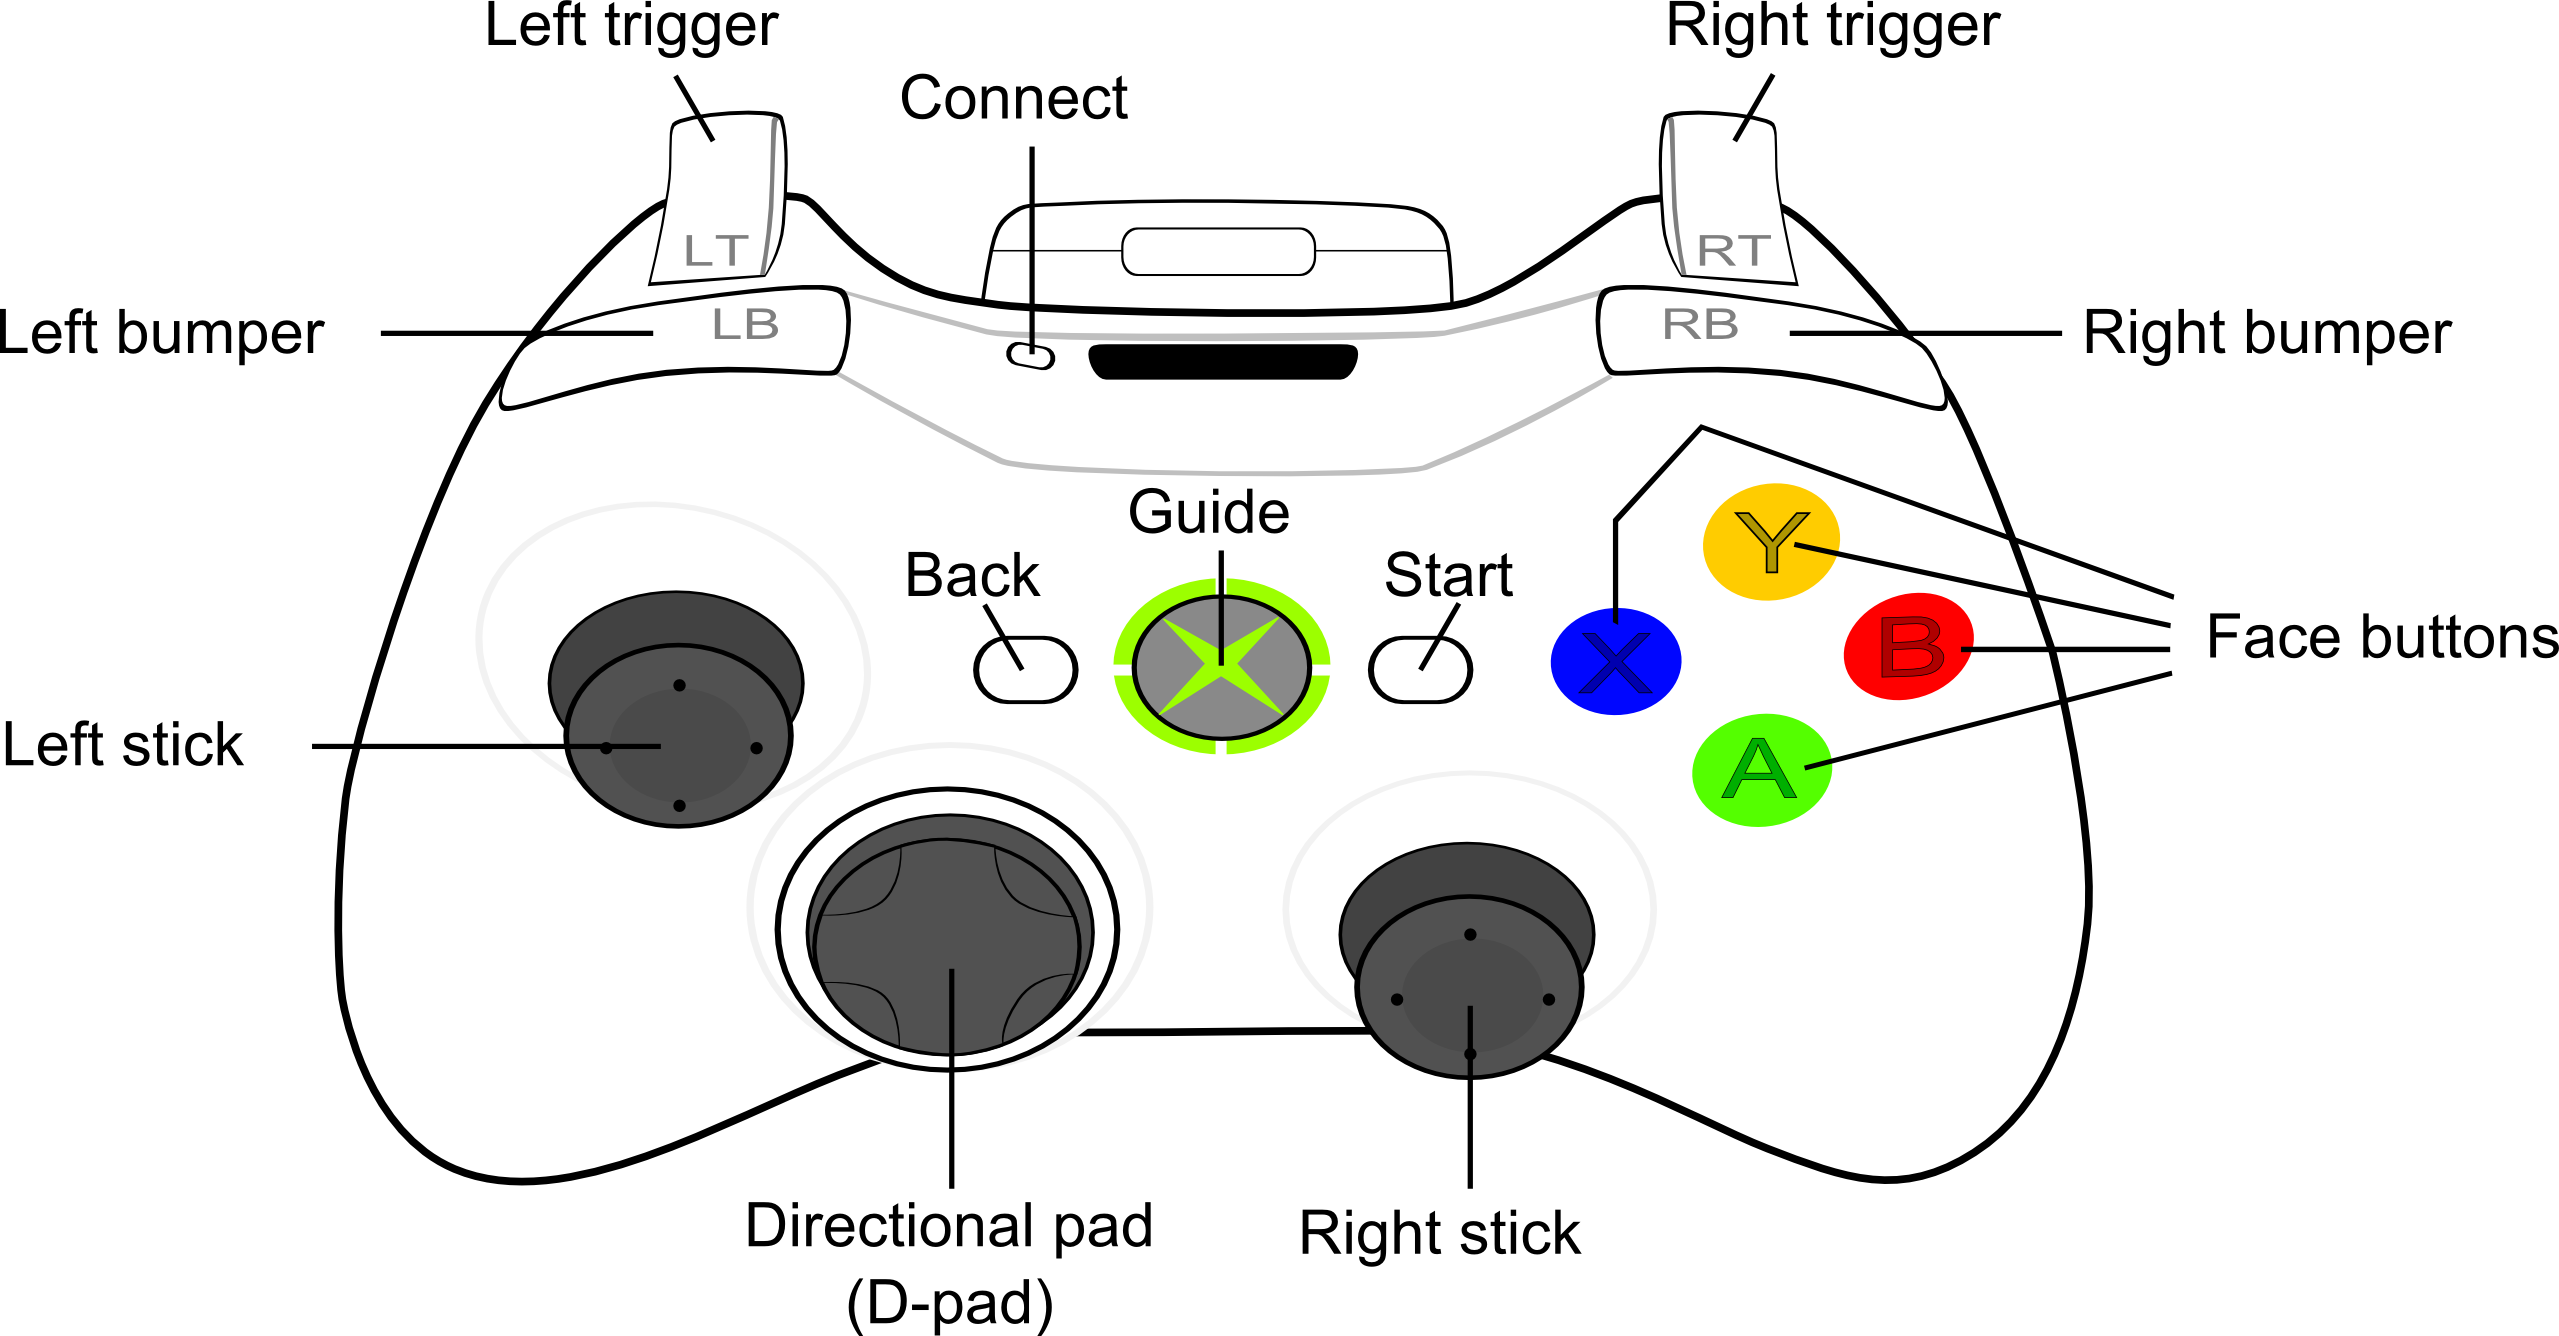
\includegraphics[width=12cm]{360.png}
	\caption{A diagram showing the layout of the Microsoft Xbox 360 Controller \cite{360_controller}. In the case of this control system, the left and right analogue sticks are used to input linear and angular motions respectively.}.
	\label{fig:xbox_360}
\end{figure}

The \texttt{joy} package contains one node named \texttt{joy\_node}. This node parses joystick input data, converts that data into standard \texttt{Joy} messages, and then broadcasts it through a \texttt{joy} topic relative to itself \cite{ros_wiki_joy}. The specification for the \texttt{Joy} message can be seen in \autoref{fig:joy_msg} and some example output from the \texttt{joy} topic can be seen in \autoref{fig:joy_example}. Additionally, \texttt{joy\_node} accepts a \texttt{dev} parameter which specifies where it should read joystick data from. If no parameter is set, the node will read data from \texttt{/dev/input/js0} which is the first controller connected to the system. 

\begin{figure}[!h]
	\centering
	\begin{tabular}{ r r p{10cm} }
		\textbf{Name} & \textbf{Type} & \textbf{Description} \\
		\hline

		\texttt{axes} & 
		\texttt{float32[]} &
		An array of floating point numbers indicating the current position of each axes on the controller, ranging from -1 to 1. An analogue stick like on the controller shown in \autoref{fig:xbox_360} will consist of two axes, one for the X position and the other for the Y position. \\
		
		\texttt{buttons} & 
		\texttt{int32[]} & 
		An array of integers indicating the state of each button on the controller. A value of 1 indicates that the button is currently pressed, while a value of 0 indicates the opposite. \\
	\end{tabular}
	\caption{The specification for the \texttt{Joy} message as used by the \texttt{joy\_node} and \texttt{gamepad\_controller} nodes. The message also contains a \texttt{header} field but is omitted for brevity.}
	\label{fig:joy_msg}
\end{figure}

\begin{figure}[!h]
	\centering
	\begin{lstlisting}
	axes:    [0.0, 0.0, 1.0, 0.0, 0.0, 1.0, 0.0, 0.0]
	buttons: [1, 0, 0, 0, 0, 0, 0, 0, 0, 0, 0]
	---
	axes:    [-1.0, 0.0, 1.0, 0.0, 0.0, 1.0, 0.0, 0.0]
	buttons: [0, 0, 0, 0, 0, 0, 0, 0, 0, 0, 0]
	---
	axes:    [0.0, 0.0, 1.0, 0.5, 0.0, 1.0, 0.0, 0.0]
	buttons: [0, 0, 0, 0, 0, 0, 0, 0, 0, 0, 0]
	\end{lstlisting}
	\caption{Some example output from the \texttt{joy} topic as provided by the \texttt{rostopic} utility. The message header has been omitted for brevity. The first message shows all axes it rest while the \emph{A} button on the controller is pressed. The second message shows the left analogue stick pushed all the way to the left with no buttons pressed. The third message shows the right analogue stick pushed halfway upwards with no buttons pressed.}
	\label{fig:joy_example}
\end{figure}

The implemented \texttt{gamepad\_controller} node listens on this \texttt{joy} topic for any controller movements. Once received, the node will send a \texttt{Twist} message to the \texttt{/cmd\_vel} topic as required by the locomotion controller. The \emph{y axis} of the left analogue, at index 1 in the axes array, is used stick for linear motion and the \emph{x axis} of the right analogue stick, in index 3 in the axes array, is used for angular motion. A ``deadzone'' had to be set on any axis movements as the analogue sticks on the controller tend not to center exactly on a (0, 0) value, causing the robot to move even if the user was not touching them in any way. Instead, movement commands will only be sent if either of the axes is moved by at least one quarter of the range (i.e., $|x| \geq 0.25$).

%%%%%%%%%%%%%%%%%%%%%%%%%%%%%%%%%%%%%%%%%%%%%%%%%%%%%%%%%%%%%%%%%%%%%%%%%%%%%%%%%%%%%%%%%%%%%%%%%%%%

\section{Sensing}

openni2 originally, ccny\_rgbd \cite{ccny_rgbd} provides some clean up features.

\subsection{Visual Odometry}

ccny\_rgbd \cite{ccny_rgbd} was used.

\subsection{Environment Mapping}

ocotomap

\subsubsection{Alternatives}

SLAM, but expects laser scan.

%%%%%%%%%%%%%%%%%%%%%%%%%%%%%%%%%%%%%%%%%%%%%%%%%%%%%%%%%%%%%%%%%%%%%%%%%%%%%%%%%%%%%%%%%%%%%%%%%%%%

\section{Navigation}

Built in stack.

\subsection{Path Planning}